\newthought{\textbf{Salsabila Irmanda - 2020903430048 - TRKJ 3B}}

\newday{\textbf{1 - 2 Desember 2022} - Instalasi dan Konfigurasi Hadoop}
\begin{enumerate}
\item Kendala dan Solusi\\
\begin{enumerate}
\item Saat melakukan percobaan instalasi hadoop terdapat kendala yaitu saat melakukan extrak file hadoop, solusi yang digunakan yaitu memberikan ukuran ruang lebih besar saat membuat os ubuntu
\item Melakukan konfigurasi apache hadoop pratikan mengalami kendala pada perintah format HDFS. solusi yang digunakan yaitu mengecek lagi file - file konfigurasi hadoop hingga tidak ada lagi kesalahan
\end{enumerate}
% jelaskan kendala dan penyebab yang dialami saat mengikuti praktikum serta solusi atau langkah-langkah yang telah dilakukan

\item Kesimpulan \\
Adapun kesimpulan yang diperoleh yaitu tahap instalasi dan konfigurasi hadoop telah berhasil. untuk mengecek hadoop service dengan perintah jps.
% berikan kesimpulan dari praktikum yang telah dikerjkan
\begin{figure}[!ht]
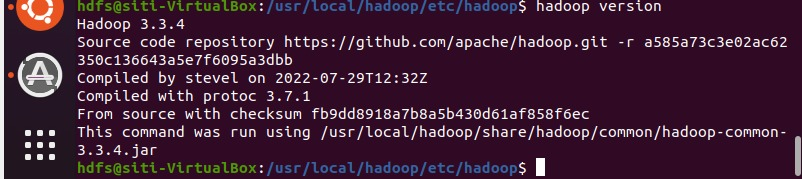
\includegraphics[width=.8\textwidth]{SalsabilaIrmanda/1}
\caption{localhost:8088}
\label{gam:perkuliahan-22-09}
\end{figure}

\newpage
\begin{figure}[!ht]
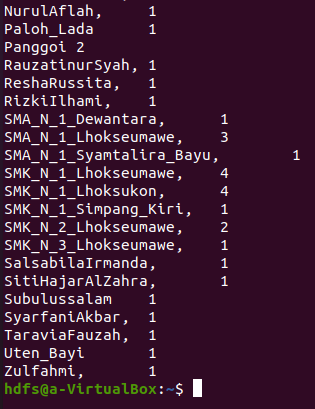
\includegraphics[width=\textwidth]{SalsabilaIrmanda/2}
\caption{localhost:9870}
\label{gam:perkuliahan-22-09}
\end{figure}
\end{enumerate}


\newday{\textbf{8 Desember 2022} - WordCount bawaan Hadoop}
\begin{enumerate}
\item Kendala dan Solusi \\
Saat melakukan percobaan program Word Count Hadoop tidak mengalami kendala. 
% jelaskan kendala dan penyebab yang dialami saat mengikuti praktikum serta solusi atau langkah-langkah yang telah dilakukan
\item Kesimpulan \\
setelah melanjutkan percobaan dan mengikuti semua langkah hingga selesai pratikan berhasil menjalankan ouput program wordcount bawaan hadoop. 

% berikan kesimpulan dari praktikum yang telah dikerjkan
\begin{figure}[!ht]
\includegraphics[width=\textwidth]{SalsabilaIrmanda/langkah6&7}
\caption{Hasil perhitungan Wordcount bawaan hadoop berdasarkan output}
\label{gam:perkuliahan-08-12}
\end{figure}
\end{enumerate}

\newday{\textbf{9 Desember 2022} - WordCount dengan Java}
\begin{enumerate}
\item Kendala dan Solusi \\
Terdapat kendala saat melakukan cek hasil pada program wordcount dengan java, solusi nya yaitu harus menjalankan hadoop service. 
% jelaskan kendala dan penyebab yang dialami saat mengikuti praktikum serta solusi atau langkah-langkah yang telah dilakukan

\item Kesimpulan \\
percobaan yang telah dilakukan yaitu melakukan proses membuat program, menyiapkan data, meng-compile program hingga menjalankan program dan berhasil menampilkan hasilnya.
% berikan kesimpulan dari praktikum yang telah dikerjkan

\begin{figure}[!ht]
\includegraphics[width=\textwidth]{SalsabilaIrmanda/langkah9}
\caption{hasil program wordcount java 9}
\label{gam:hasil}
\end{figure}

\begin{figure}[!ht]
\includegraphics[width=\textwidth]{SalsabilaIrmanda/langkah10}
\caption{hasil program wordcount java 10}
\label{gam:hasil}
\end{figure}
\end{enumerate}

\newpage
\newday{\textbf{15 Desember 2022} - Instalasi Apache Spark(PySpark)}
\begin{enumerate}
\item Kendala dan Solusi
\newline pada percobaan instalasi apache spark, saat menjalankan perintah verifikasi hasil intalasi tidak muncul. solusi yang digunakan yaitu mengecek kembali program pada langkah ke 4.
% jelaskan kendala dan penyebab yang dialami saat mengikuti praktikum serta solusi atau langkah-langkah yang telah dilakukan

\item Kesimpulan
setelah melakukan pengecekan hingga tidak terdapat lagi kesalahan maka pyspark berhasil dijalankan.
% berikan kesimpulan dari praktikum yang telah dikerjkan
\begin{figure}[!ht]
\includegraphics[width=\textwidth]{SalsabilaIrmanda/installspark}
\caption{hasil verifikasi instalasi spark}
\label{gam:hasil}
\end{figure}
\end{enumerate}

\newday{\textbf{16 Desember 2022} - Program WordCount dengan Python}
\begin{enumerate}
\item Kendala dan Solusi
\newline pada praktikum ini, pratikan tidak mendapat kendala. 

% jelaskan kendala dan penyebab yang dialami saat mengikuti praktikum serta solusi atau langkah-langkah yang telah dilakukan

\item Kesimpulan
\newline setelah melakukan percobaan dari tahap awal sampai selesai, kemudian melakukan pengecekan hasil dan melihat hasil word count dengan python. jika hasilnya muncul dan sesuai maka pratikan telah berhasil melakukan percobaan word count dengan python.
% berikan kesimpulan dari praktikum yang telah dikerjkan
\begin{figure}[!ht]
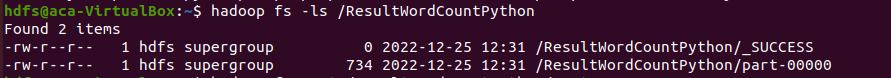
\includegraphics[width=\textwidth]{SalsabilaIrmanda/cekhasil wordcount python}
\caption{pengecekan hasil program wordcount dengan python}
\label{gam:cekhasil}
\end{figure}

\newpage
\begin{figure}[!ht]
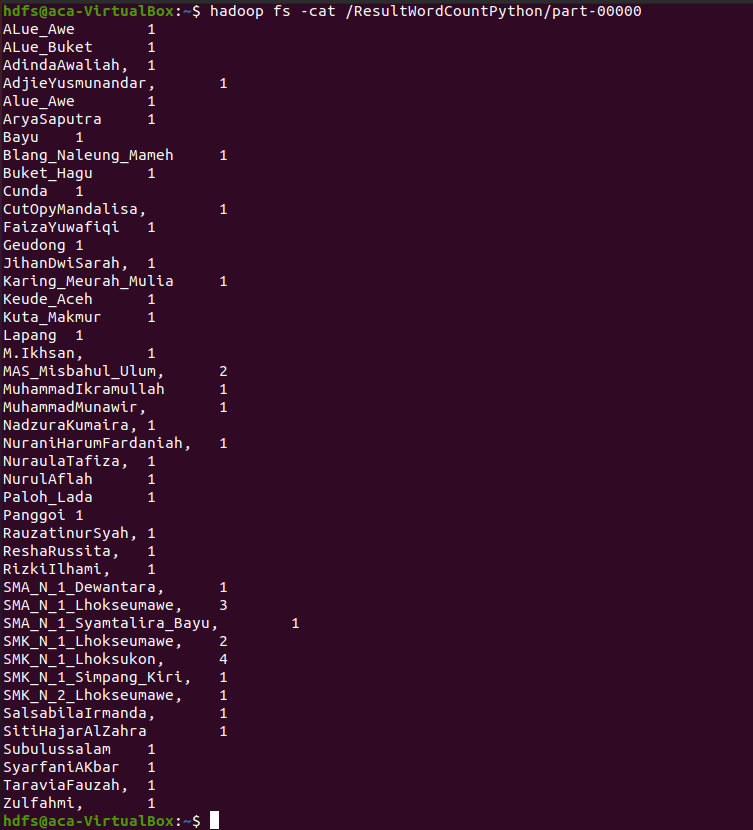
\includegraphics[width=\textwidth]{SalsabilaIrmanda/hasilwordcount python}
\caption{hasil program wordcount dengan python}
\label{gam:hasil}
\end{figure}
\end{enumerate}

\newday{\textbf{22 Desember 2022} - Program WordCount dengan PySpark}
\begin{enumerate}
\item Kendala dan Solusi
\newline Pada percobaan program wordcount dengan pyspark ini pratikan tidak mengalami kendala.
% jelaskan kendala dan penyebab yang dialami saat mengikuti praktikum serta solusi atau langkah-langkah yang telah dilakukan

\item Kesimpulan
\newline Setelah melakukan percobaan dari tahap awal sampai selesai,pratikan telah berhasil melakukan percobaan wordcount dengan pyspark.
% berikan kesimpulan dari praktikum yang telah dikerjkan
\begin{figure}[!ht]
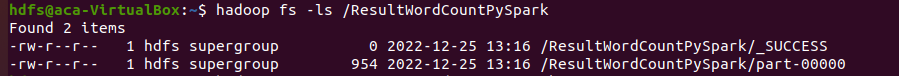
\includegraphics[width=\textwidth]{SalsabilaIrmanda/cekhasil wordcount pyspark}
\caption{pengecekan hasil program wordcount dengan pyspark}
\label{gam:cekhasil}
\end{figure}

\newpage
\begin{figure}[!ht]
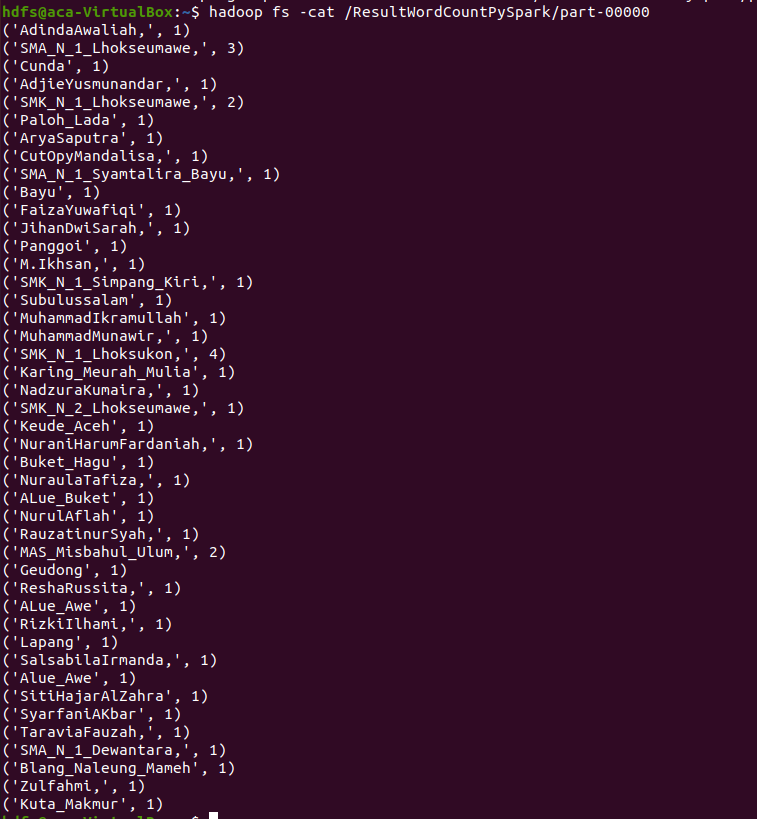
\includegraphics[width=\textwidth]{SalsabilaIrmanda/hasilwordcount pyspark}
\caption{hasil program wordcount dengan pyspark}
\label{gam:hasil}
\end{figure}
\end{enumerate}

\newday{\textbf{23 Desember 2022} - Program Machine Learning dengan PySpark}
\begin{enumerate}
\item Kendala dan Solusi
\newline pada percobaan machine learning dengan pyspark pratikan mengalami kendala yaitu saat install python3, solusi yang digunakan yaitu pratikan menginstall dengan cara masuk ke root manual dengan menambahkan perintah sudo dpkg --configure -a
% jelaskan kendala dan penyebab yang dialami saat mengikuti praktikum serta solusi atau langkah-langkah yang telah dilakukan

\item Kesimpulan
\newline Pratikan melanjutkan percobaan dan mengikuti semua langkah - langkah modul hingga selesai dan pratikan berhasil load data, menentukan nilai K dengan metode silhouette, dan menampilkan hasil clustering dengan PCA.
% berikan kesimpulan dari praktikum yang telah dikerjkan
\begin{figure}[!ht]
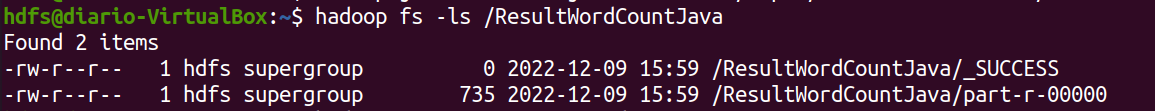
\includegraphics[width=\textwidth]{SalsabilaIrmanda/hasil1}
\caption{hasil load data}
\label{gam:hasil}
\end{figure}

\begin{figure}[!ht]
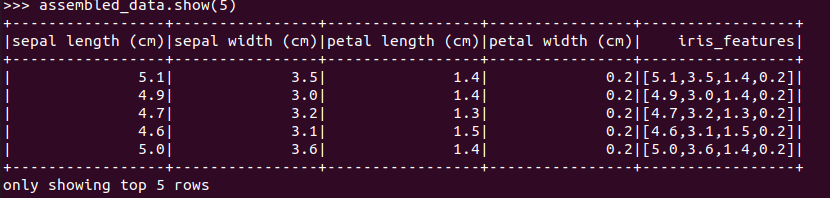
\includegraphics[width=\textwidth]{SalsabilaIrmanda/hasil2}
\caption{hasil penentuan nilai K dengan metode silhouette}
\label{gam:hasil}
\end{figure}

\begin{figure}[!ht]
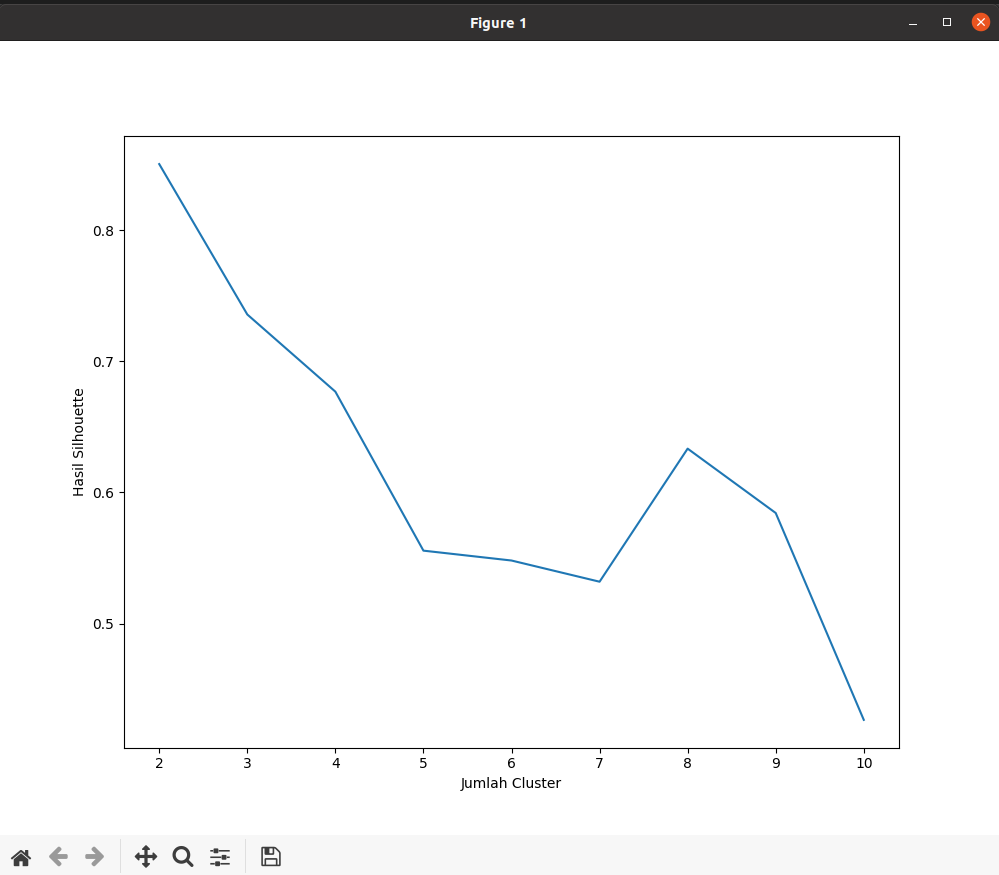
\includegraphics[width=\textwidth]{SalsabilaIrmanda/grafik1}
\caption{grafik penentuan nilai K dengan metode silhouette}
\label{gam:hasil}
\end{figure}
\newpage
\begin{figure}[!ht]
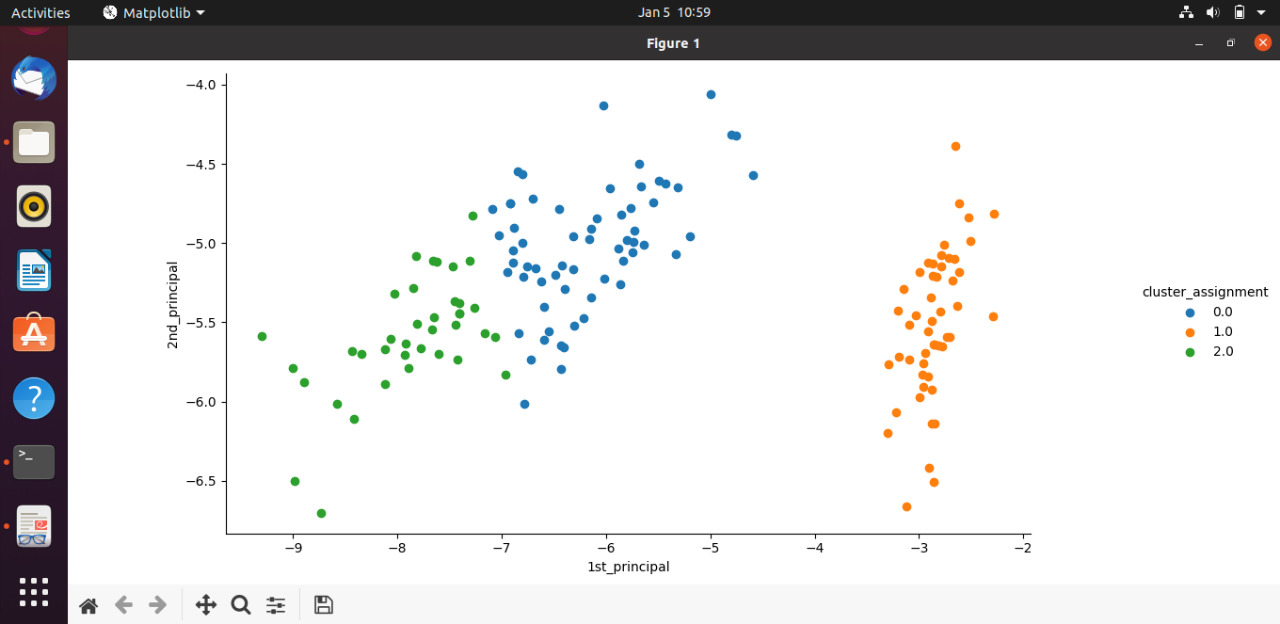
\includegraphics[width=\textwidth]{SalsabilaIrmanda/grafik2}
\caption{hasil clustering dengan PCA}
\label{gam:hasil}
\end{figure}
\end{enumerate}